\subsection{Convolutional networks} \label{hmc_cnn}

Convolutions were originally designed for image. However, they can also be used on text, to reduce the size of the data while keeping relevant information. Doing so helps with regularization, as the complexity of the data is reduced. \cite{kim2014convolutional} proposed one-dimensional convolutions and pooling for text input, which are now the common approach. We present these operations here, before discussing two relevant implementations of convolutions for \acrshort{hmc} tasks.

\subsubsection{Convolutions for text}

When applied to text, convolutions are usually one-dimensional. In contrast, convolutions are two-dimensional when applied to images. This has to do with the structure of text and images. The words in a text are ordered across one dimension, whereas the pixels of an image are located in a two-dimensional space. Convolutions extract features from multiple word vectors at a time. Therefore, the result doesn't necessarily change the number of vectors; it affects the number of dimensions.

The number of filters is the number of features we want to extract from each word vector, when considering its surroundings. How large the considered context is, is defined by the kernel size. The number of vectors can be ensured to remain constant with padding, which is done in the original implementation. A single convolution receives $k$ one-dimensional vectors of size $n$ and outputs a single one-dimensional vector of size $m$. $k$ is the kernel size, which defines how many words are considered by each convolution, and $m$ is the number of filters (what PyTorch refers to as output channels), which defines how many vectors remain after the convolutional layer.

\subsubsection{Pooling for text}

Pooling is used to reduce the size of the data while keeping the most important information. The original implementation uses the most popular form of pooling, called max-pooling. Max-pooling takes the maximum over each dimension of the data, thus reducing the number of word vectors. Recall that each dimension represents a feature. The kernel size of the pooling layer defines how many word vectors are considered at a time. For instance, if the kernel size is two, the number of vectors is halved, as the maximum value for all dimensions of each pair of word vectors is kept.

\subsubsection{CNN for HMC} \label{hmc_gargiulo}

\cite{gargiulo2019deep} uses a convolutional model and various embedding methods to index medical documents with MeSH subjects, a hierarchical set of 27,775 subjects regarding Medicine and Biology. Their dataset consists of over eleven million documents from PubMed.

Their architecture comprises three stages. In the first stage, the words are replaced by vectors. The authors try different embedding methods, including the pre-trained fasttext vectors and a normalization pipeline that lower-cased and tokenized the texts, as well as removing numbers punctuation signs, numbers and stopwords. The remaining words were then lemmatized. This is not really an embedding method, but does play an important role in the quality of the embeddings. They experimented with five different embedding methods and various combinations of them. They concluded that the normalization pipeline significantly increased the performance of the model, whereas concatenating different embeddings usually decreased the model's accuracy.

The second stage of their architecture, termed \textit{feature extraction module}, consists of two convolutional layers, followed by max-pooling layers, which reduce the dimensionality of the data while hopefully retaining as much information as possible. A dropout layer with 1 \% discard probability ends this stage, as a regularization method. Interestingly, their first max-pooling layer is said to have size 1, meaning that the maximum value is picked for each window of size 1. This of course is useless; the input to the layer is forwarded without any modifications. We have looked in related work for an explanation, but unfortunately couldn't find any. A previous paper of the first author shows a similar convolutional architecture, but where the max-pooling layer has size 2. This is also the case for the second max-pooling layer in this architecture.

The third and final stage of their architecture is where the indexing occurs. It comprises two fully connected layers, where the size of the output layer equals the number of labels. The first layer has a Rectified Linear Unit (ReLU) activation function and the second, a sigmoid function. The second and third stages, which are the actual neural network model, are depicted in figure \ref{fig:gargiulo}. The first convolutional layer receives a matrix with $N$ words, each of $D$ dimensions. The authors chose 400 as the number of words, padding documents with less words and truncating those with more.

\begin{figure}
    \centering
    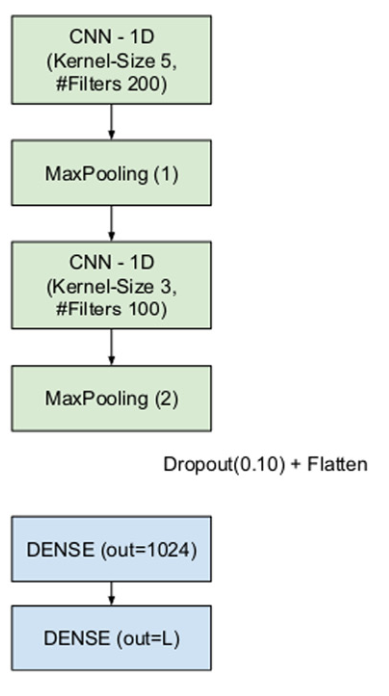
\includegraphics[width=.3\textwidth]{figures/hmc/gargiulo.png}
    \caption{Convolutional architecture for HMC from \cite{gargiulo2019deep}.}
    \label{fig:gargiulo}
\end{figure}

The model is trained with the \acrfull{bce} loss function, which is often used in multi-label settings because each label is treated independently. The model is trained with \acrfull{sgd}, with a mini-batch size of 10, momentum 0.9 and Nesterov accelerated gradients. Besides the comparison of embedding methods, their contribution includes a regularization method, called Hierarchical Label Set Expansion (HLSE), which ensures that if a subject is assigned to a document, its parents are assigned as well. This regularization method reduces the noise in the data, but also increases the complexity of the task, as more labels have to be predicted. However, their experiments conclude that HLSE does increase model accuracy.
